\phantomsection

\chapter{State of the art}
\markboth{State of the art}{}

\begin{citazione}
\end{citazione}
\newpage

\section{Simulation tools comparison} { \setstretch{1.3}
Simulation tools play a critical role in various domains of cloud computing. They offer researchers and infrastructure designers a virtual environment to work in, eliminating the expenses associated with physical infrastructure. Over time, several authors have conducted comparative studies to assess different simulators and highlight their unique characteristics, assisting users in selecting the most suitable option for their specific context. In this section, we will discuss about several cloud simulators that have been studied by the researchers focusing on their main strengths and drawbacks as well as the problems they address. Since our primary focus is to identify a simulator that is well-suited for energy consumption metrics extraction we will prioritize features that ensure the accuracy of the simulations in order to make this work relevant in real scenarios. The following argument is based on several previous surveys, namely: \emph{N. Mansouri, et al.} \cite{mansouri2020cloud}, \emph{P. Suryateja} \cite{suryateja2016comparative}, \emph{D. Perez Abreu, et al.} \cite{abreu2020comparative}, \emph{Khaled M. Khalil, et al.} \cite{khalil2017cloud}, \emph{Nimisha Patel
\& Hiren Patel} \cite{patel2016comprehensive}.
 
\subsubsection{CloudSim}
When it comes to cloud simulators it is impossible to overlook \emph{CloudSim} \cite{calheiros2011cloudsim}, as it is one of the most widely used \emph{event-driven} tools among researchers. A search for the keyword "\emph{CloudSim}" on the \emph{Scopus} platform yields 2020 results (this search was performed in May 2023), indicating its popularity and widespread adoption in the research community. Over the years, several simulators based on \emph{CloudSim} have been proposed. This tool, written in \emph{Java}, is comprehensive and highly extensible, making it a popular choice in the Cloud research field.
One notable feature is its virtualization engine, which allows the creation and management of virtualization services on a network node. Additionally, \emph{CloudSim} provides the capability to allocate machine cores in two different ways: space-shared and time-shared.
In space-shared allocation, the machine is divided into a set of cores, and each core is assigned to a single job until it is completed. On the other hand, in time-shared allocation, multiple jobs can be assigned to a single core, and each job is executed for a certain period of time before another job is chosen.
Overall, \emph{CloudSim} offers researchers a comprehensive and flexible platform to simulate and study virtualization and resource allocation techniques \cite{mansouri2020cloud}.
Architecture of \emph{CloudSim} is shown in figure \ref{fig:cloudsim_arch}. It is composed by three layers, described below:
\begin{itemize}
    \item \textbf{CloudSim core simulation engine}: initially implemented through the discrete event simulation engine \emph{SimJava} that supports functionalities such as queuing, processing of events, creation of Cloud system entities, communication between components and management of the simulation clock (\cite{calheiros2011cloudsim}), it has been replaced with an engine that provides some advanced operations;
    \item \textbf{CloudSim simulation level}: it provides various interfaces and services that allow to model and simulate Cloud-based data center environments; 
    \item \textbf{User code}: it allows to set up various simulation parameters such as number of machines, their specification, number of tasks and broker scheduling policies.
\end{itemize}
\begin{figure}[h]
    \centering
    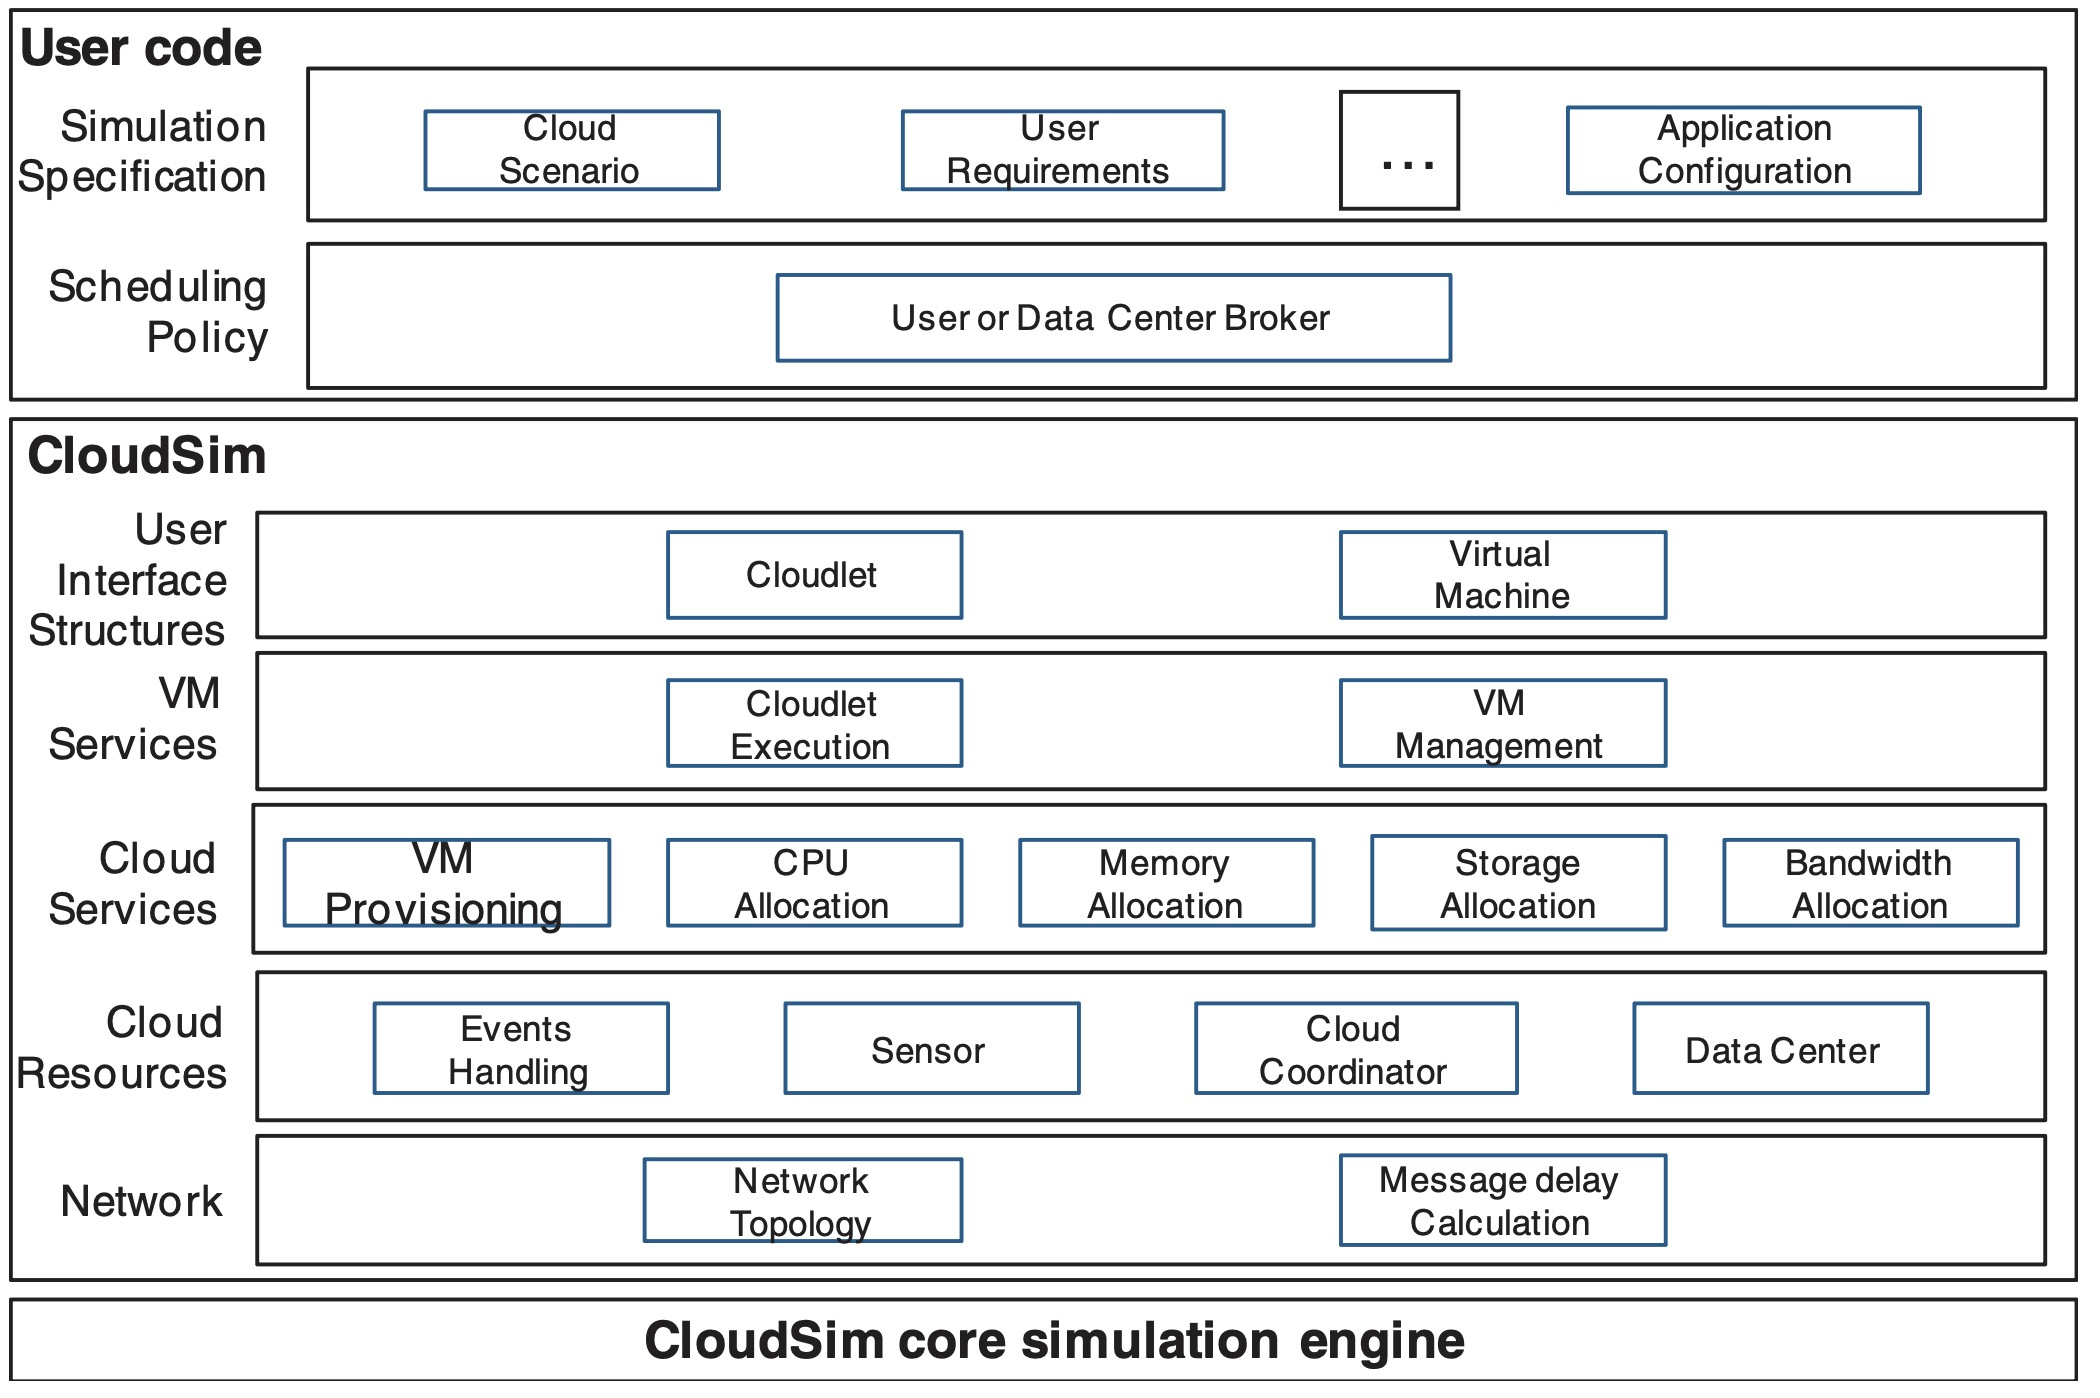
\includegraphics[width=0.5\textwidth]{capitoli/images/cloudsim_arch.jpeg}
    \caption{CloudSim architecture}
    \label{fig:cloudsim_arch}
\end{figure}
\subsubsection{NetworkCloudSim}
\emph{NetworkCloudSim} \cite{garg2011networkcloudsim} implements a network layer and  provides several communication models, including message-based, packet-based and flow-based models. It also offers an accurate evaluation of the scheduling of machines in the data center. Finally, it provides a basic energy model of the data center, although it does not extensively focus on energy efficiency and it does not provide a packet-level network model \cite{mansouri2020cloud} \cite{patel2016comprehensive}.
\subsubsection*{CloudAnalyst}
CloudAnalyst \cite{wickremasinghe2010cloudanalyst} makes simulation work easier as it provides a \emph{GUI}. One of the notable features of CloudAnalyst is the ability to obtain information about the geographical location of users and data centers. The simulator also offers a set of metrics based on response time and request processing. However, it does not implement a complete communication model based on the \emph{TCP/IP} protocol and it provides a poor energy model \cite{mansouri2020cloud}. 
\subsubsection{EMUSim}
\emph{EMUSim} \cite{calheiros2013emusim} includes an emulation and a simulation environment. The simulator is able to get profiling data about the running application behavior through the emulation environment; these data are used to build a simulation environment. However, the emulation environment strongly limits scalability and makes the simulator not suitable for large workload scenarios \cite{mansouri2020cloud}. 
\subsubsection*{CDOSim}
\emph{CDOSim} \cite{fittkau2012cdosim} integrates \emph{CloudSim} simulator and \emph{CloudMIG} framework. This simulator adopts a scaling technique that assigns a new virtual machine when CPU usage exceeds a specific threshold.  It provides a set of client-centric metrics, allowing developers to compare different solutions based on various deployment parameters. Another noteworthy feature is the presence of a benchmark module that detects the impact of choosing a specific architecture on application performance. However, the communication model employed by CDOSim is overly simplistic and strongly limits large-scale applications \cite{mansouri2020cloud}.
\subsubsection*{TeachCloud}
TeachCloud \cite{jararweh2013teachcloud} is designed to be suitable for students who want to have some practical experience with Cloud Computing simulation, covering aspects such as networking, Service Level Agreement contraints, web-based applications, Service Oriented Architecture, virtualization, and so on. Through a user-friendly \emph{GUI} it allows to design several network architectures in addition to the pre-existing ones. This simulator lacks realism in various aspects since it is mainly designed for academic purposes. For example, the simulator does not consider the possibility of faults in the data center, preventing developers from studying the impact of faults on application usage \cite{mansouri2020cloud} \cite{patel2016comprehensive}.
\subsubsection*{DartCSim}
DartCSim \cite{li2012dartcsim} provides a simple \emph{GUI} that allows users to set various simulation parameters, such as the characteristics of the data center and the network topology. These parameters can be imported and exported at any level of the simulation and can be set for individual CPUs or the entire data center. However, this tool lacks a comprehensive energy model, which prevents developers from implementing strategies aimed at improving data center efficiency \cite{mansouri2020cloud}.
\subsubsection*{DartCSim+}
\emph{DartCSim+} \cite{li2013dartcsim+} aims to enhance \emph{CloudSim} by introducing an energy model and a network model, allowing developers to design power-aware scheduling algorithms. However, this simulator does not include a cost model and lacks security features, which prevents developers from analyzing the security aspects of the data center \cite{mansouri2020cloud}.
\subsubsection*{ElasticSim}
\emph{ElasticSim}'s \cite{cai2017elasticsim} main feature is the resources runtime auto-scaling based on stochastic modeling that allows developers to design efficient scheduling algorithms. However, this simulator provides a poor energy consumption model and it cannot simulate security-related experiments. \cite{mansouri2020cloud}
\subsubsection*{FederatedCloudSim}
FederatedCloudSim \cite{kohne2014federatedcloudsim} aims to provide developers with the capability to test various types of cloud federations. This simulator builds upon the functionalities of \emph{CloudSim} and expands them by incorporating features such as Service Level Agreement management, workload generation, event logging, scheduling, and brokering. While the simulator offers comprehensive functionality for modeling and simulating cloud federations, it does not provide specific insights into the energy consumption of each data center in the federation \cite{mansouri2020cloud}.
\subsubsection*{FTCloudSim}
FTCloudSim \cite{zhou2013ftcloudsim} is primarily designed to simulate reliability mechanisms in cloud services. It offers implementations of various reliability mechanisms, allowing developers to analyze and evaluate the performance of these mechanisms. The simulator also includes fault generation services, which enable the generation of faults based on specific probability distributions. However, one drawback of FTCloudSim is its simplified energy consumption model, which can impact the assessment of energy-efficient strategies or algorithms \cite{mansouri2020cloud}.
\subsubsection*{WorkflowSim}
\emph{WorkflowSim} \cite{chen2012workflowsim} provides a platform for studying the performance impact of different job clustering strategies in a data center. It achieves this by implementing various workflow scheduling methods. However, WorkflowSim has limitations when it comes to simulating data-intensive applications. It does not consider the delays caused by input-output operations, which are crucial in such scenarios. Additionally, the supported fault model in WorkflowSim is limited, which can affect the realism of simulations. As a result, the accuracy and realism of simulations involving data-intensive applications may be compromised \cite{mansouri2020cloud}. 
\subsubsection*{CloudReports}
\emph{CloudReports} \cite{teixeira2014cloudreports} provides developers with a user-friendly \emph{GUI} that allows them to manage various aspects of the data center and access detailed reports on resource utilization, virtual machine allocation, and energy consumption. The simulator offers valuable insights into these metrics, enabling developers to analyze and optimize resource usage and energy efficiency.
However, one limitation of \emph{CloudReports} is the absence of a dedicated security layer. This means that developers cannot explore and evaluate the security characteristics of the data center using this simulator \cite{mansouri2020cloud}.
\subsubsection*{CEPSim}
CEPSim \cite{higashino2015cepsim} models various \emph{Complex Event Processing (CEP)} environments \cite{luckham1998complex} where users can define queries using different proprietary languages and model the execution flow using a directed acyclic graph. The simulator implements various load scheduling algorithms, allowing developers to evaluate queries under different load conditions. However, one limitation of \emph{CEPSim} is that it does not consider network consumption. As a result, the simulator may not provide a comprehensive analysis of energy consumption from a network perspective. Other factors such as network transmission impact on energy consumption are not explicitly taken into account \cite{mansouri2020cloud}.
\subsubsection*{DynamicCloudSim}
DynamicCloudSim \cite{bux2013dynamiccloudsim} is primarily concerned with addressing the instability of computing center parameters that can change during runtime. It specifically introduces failure models for task execution, allowing developers to define the failure rate when conducting experiments in a simulated environment. However, one limitation is that developers do not have the capability to calculate the energy consumption of the experiments accurately due to the restricted nature of the provided energy model; moreover, its failure model is strongly limited. \cite{mansouri2020cloud}. \cite{suryateja2016comparative}
\subsubsection*{CloudExp}
\emph{CloudExp} \cite{jararweh2014cloudexp} provides developers with a simple \emph{GUI} that allows easy configuration of environment parameters and monitoring of their behavior. Specifically, CloudExp enables the definition of a Service Level Agreement (SLA) based on parameters such as the number of users, service availability and cost, network performance, and security measures. Additionally, it establishes a specialized framework for cloud computing in mobile device scenarios. However, the energy model used by the simulator is simplistic and not suitable for analyzing energy-aware strategies \cite{mansouri2020cloud} \cite{khalil2017cloud}.
\subsubsection*{CM Cloud}
\emph{CM Cloud} \cite{alves2016cm} is able to estimate overall energy simulation expenses through a comparison between several providers such as \emph{Google}, \emph{Microsoft} and \emph{Amazon}. However, this simulator lacks a complete communication model, not allowing developers to define specific traffic patterns or investigate the overall impact of the traffic generated by the hosts of the network. Finally, there is no task failure model \cite{mansouri2020cloud}.
\subsubsection*{MR-CloudSim}
\emph{MR-CloudSim} \cite{jung2012mr} is based on the \emph{MapReduce} computational model \cite{dean2008mapreduce} for big data computation, allowing developers to work with data-intensive applications. One limitation is that it does not allow developers to accurately calculate service usage expenses as it does not consider file processing time and cost \cite{mansouri2020cloud}.
\subsubsection*{UCloud}
\emph{UCloud} \cite{sqalli2012ucloud} is designed to address educational purposes as it simulates cloud for universities, allowing developers to evaluate several policies in the public and private clouds. However, this simulator lacks a support for security policies and a cost model. \cite{mansouri2020cloud}
\subsubsection*{CloudSimSDN}
\emph{CloudSimSDN} \cite{son2015cloudsimsdn} is built for cloud environments based on \emph{Software Defined Networking}, namely a programmatic approach to network management \cite{benzekki2016software}. It is a scalable simulator that allows to manage energy consumption and resource policies as well as investigate several metrics such as performance. Its major drawback is that it models applications through a set of tasks and assumes long packet transmission between VMs, which can impact the granularity of application communication, making it not well-suited for works based on applications. \cite{khalil2017cloud} \cite{abreu2020comparative}
\subsubsection*{MDCSim}
\emph{MDCSim} \cite{lim2009mdcsim} is a simulation platform for multilayer data centers analysis that allows developers to investigate applications performance under different loads and tier configurations as it has low simulation overhead. \emph{MDCSim} is able to estimate several parameters, such as throughput, response time and power consumption, so developers can compare different energy policies. However, it lacks simulation realism as it does not provide a complete network model \cite{mansouri2020cloud} \cite{patel2016comprehensive}.
\subsubsection*{GDCSim}
GDCSim \cite{gupta2011gdcsim} is an open source, event-based simulator written in C, C++ and Shell, as part of the \emph{BlueTool} computer infrastructure project funded by \emph{NSF}. It is designed to analyze green data centers as it provides a simulation environment where it is possible to analyze the energy consumption of the data center in a simple and accurate way. This tool also takes into account the thermal impact of the data center, giving developers the ability to design cooling policies and energy management strategies with a particular attention to the Computational Fluid Dynamics (CFD) that allows to characterize the thermal effects and airflow patterns. However, this simulator does not consider aspects related to the security of the data center. Moreover it does not allow parallel execution of defined experiments \cite{mansouri2020cloud}.
Architecture of \emph{GDCSim} is shown in figure \ref{fig:gdcsim_arch}. It is composed by four modules:
\begin{enumerate}
    \item \textbf{BlueSim Tool}: a simulation package which integrates various software for HRMs (heat recirculation matrix) array generation;
    \item \textbf{Input/Output Management}: the interface between the user and the simulator. It takes the following inputs: job trace, Service Level Agreement, management schemes and queuing model;
    \item \textbf{Resource Management}: module that implements the following algorithms: workload management, power management, cooling management and coordinated workload, power and cooling management;
    \item \textbf{Simulator}: it provides several modules such as the queuing module, the power module, the thermodynamic module and the cooling module.
\end{enumerate}
\begin{figure}[h]
    \centering
    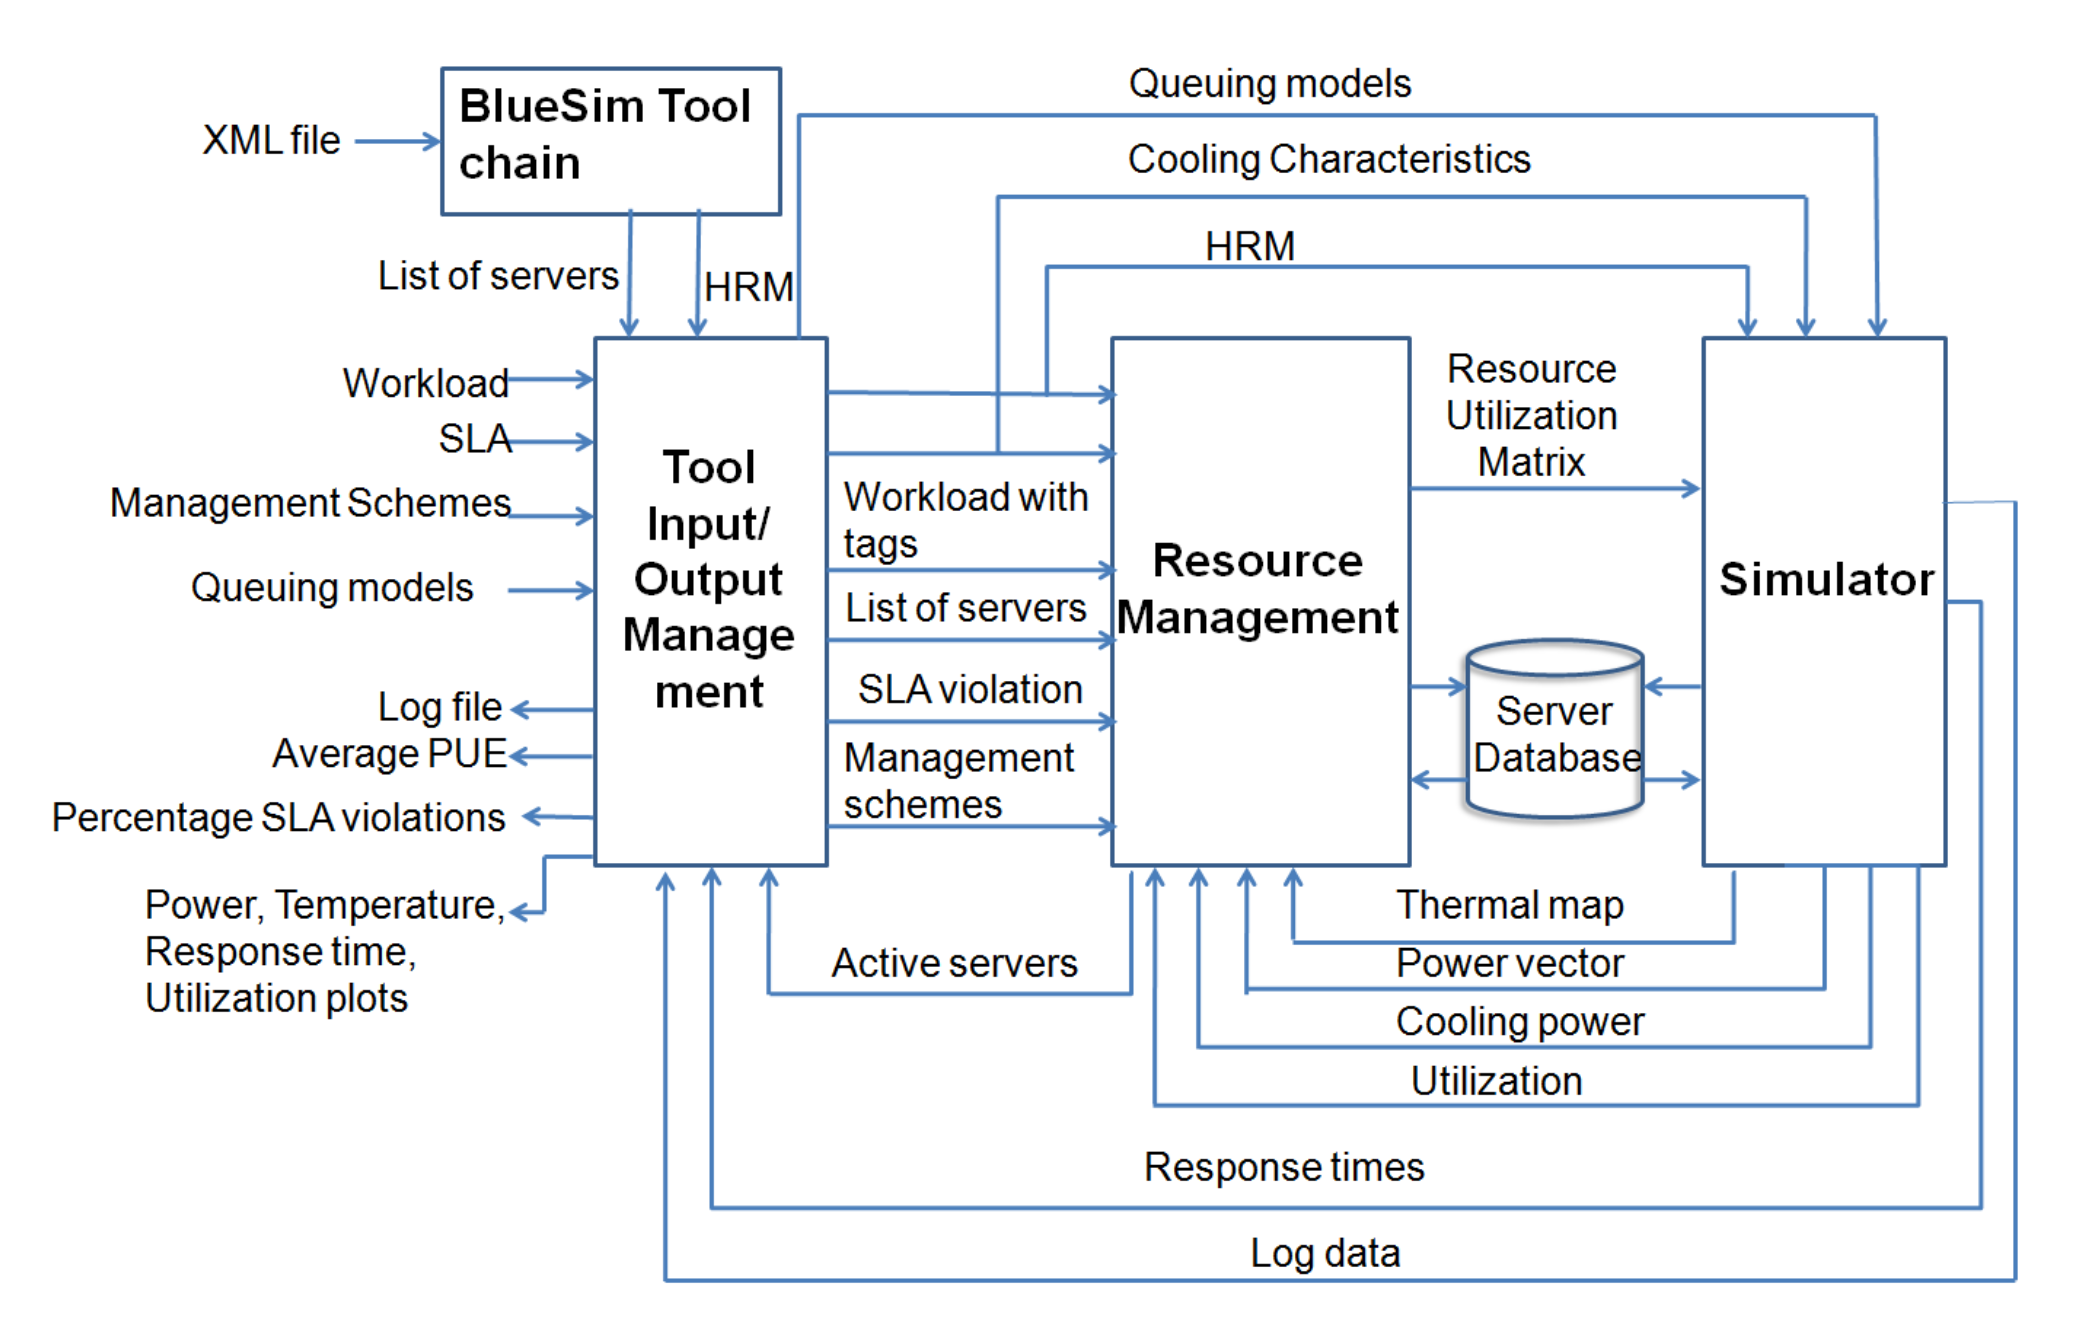
\includegraphics[width=0.5\textwidth]{capitoli/images/gdcsim_arch.png}
    \caption{Architecture of the GDCSim simulation environment}
    \label{fig:gdcsim_arch}
\end{figure}

\subsubsection*{CloudNetSim}
\emph{CloudNetSim} \cite{cucinotta2013cloudnetsim} models end-to-end communication between clients and servers. Its extensibility and modularity make it possible to integrate different modules and evaluate different VM deployment algorithms. This simulator provides a platform that allows developers to investigate resource management for realistic cloud applications. However, \emph{CloudNetSim} implements a poor energy and thermal model that makes energy management algorithms implementation difficult. \cite{mansouri2020cloud}
\subsubsection{CloudNetSim++}
\emph{CloudNetSim++} \cite{malik2014cloudnetsim++} is an open source simulator built on the top of \emph{OMNET++}, written in \emph{C++}. It introduces the concept of distributed data centers connected with physical network through various topologies. This simulation tool has a modular architecture that allows researchers to explore different aspects of data centers and to extend network topology by adding switches at the aggregation and core levels. \emph{CloudNetSim++} provides a platform to analyze energy consumption during the simulation and an energy-aware scheduler which supplies several techniques such as Dynamic Voltage and Frequency Scaling. 
\emph{CloudNetSim++} architecture is shown in figure \ref{fig:cloudnetsim++_arch} and consists of five modules:
\begin{itemize}
    \item \textbf{Pricing Policy Manager}: computes the billing cost for each user request based on the agreement;
    \item \textbf{Cloud Usage Monitor}: analyzes usage patterns;
    \item \textbf{Task Scheduling Selection Module}: determines the scheduling policy;
    \item \textbf{VM Manager}: Determines VM assignments according to the received SLA requests;
    \item \textbf{User Task Scheduler}: receives all incoming user requests and distributes them to the appropriate VMs.
\end{itemize}
\begin{figure}[h]
    \centering
    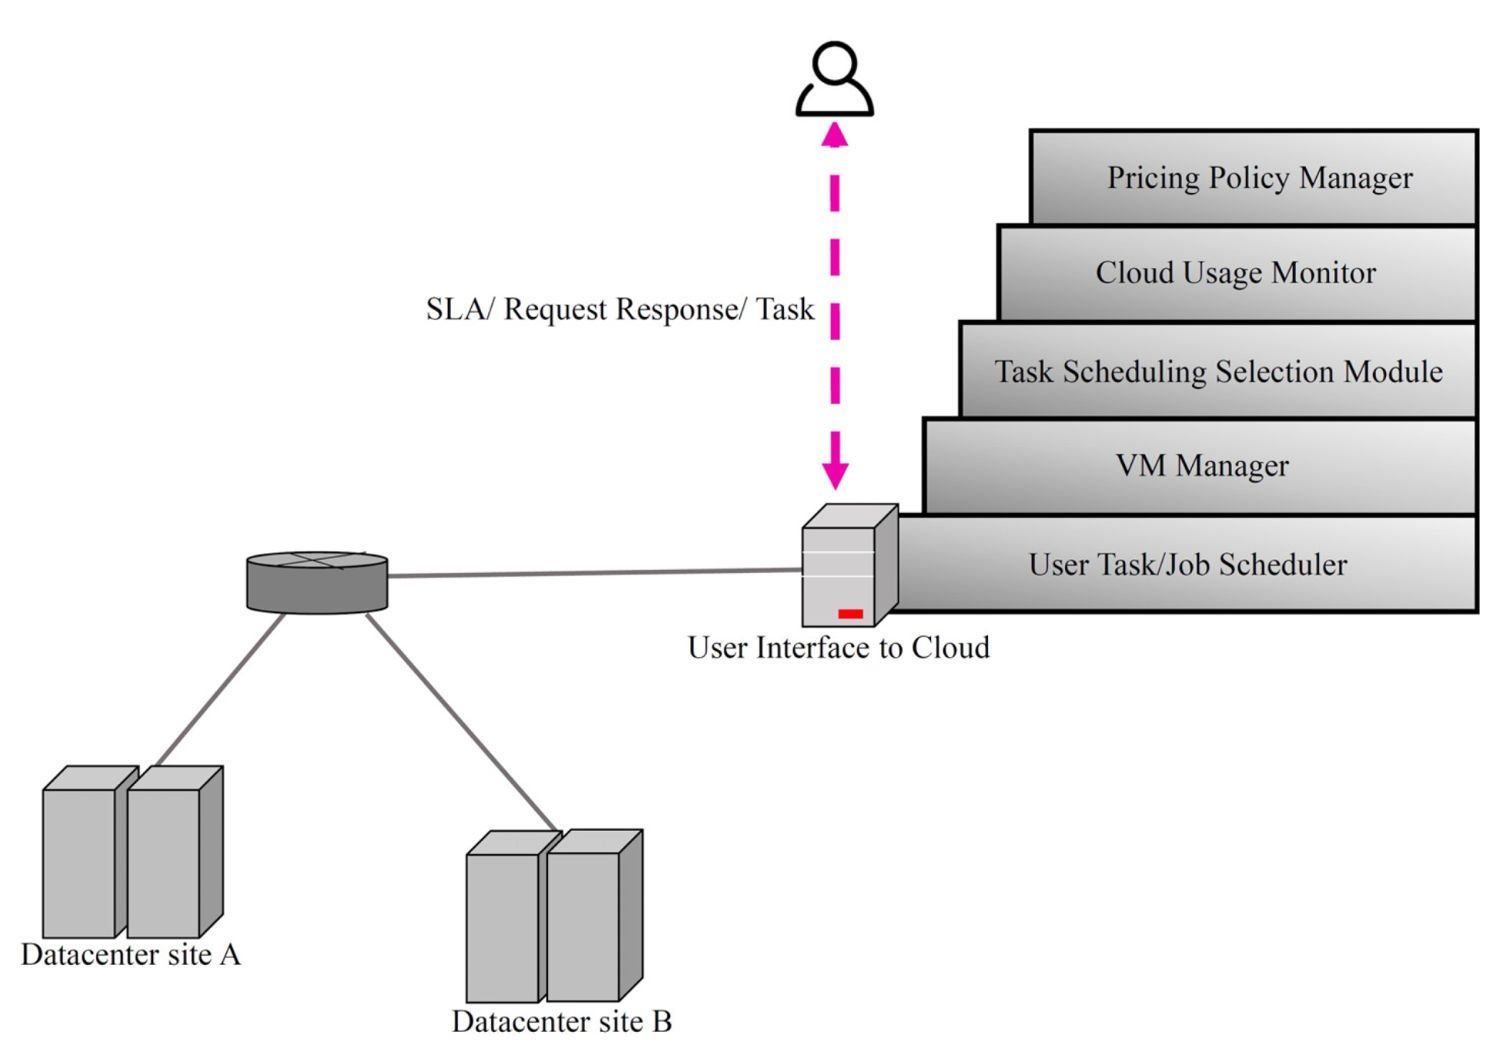
\includegraphics[width=0.5\textwidth]{capitoli/images/cloudnetsim++_arch.png}
    \caption{Architecture of the CloudNetSim++ simulation environment}
    \label{fig:cloudnetsim++_arch}
\end{figure}\subsubsection*{GreenCloud}
\emph{GreenCloud} \cite{kliazovich2012greencloud} is an open source simulation tool, written in \emph{C++} and \emph{OTcl},built on the top of \emph{NS2} that enables researchers to study the energy consumption of data centers in detail. It operates at the packet level, meaning that it simulates the behavior of individual network packets and their interactions within the TCP/IP protocol suite that is fully implemented by this simulator. The main objective of \emph{GreenCloud} is to provide insights into the energy usage of various components within a data center, including servers, switches, and network links. By accurately modeling the energy consumption patterns of these components, \emph{GreenCloud} allows users to evaluate the effectiveness of different energy-saving techniques and algorithms. However, despite its utility in energy monitoring, \emph{GreenCloud} has encountered challenges related to scalability. Simulation times in \emph{GreenCloud} tend to be relatively long, which can limit the ability to run extensive experiments or perform real-time simulations. Additionally, the simulator requires significant memory resources, which can pose constraints on the size and complexity of the simulated scenarios. These scalability limitations can make it difficult to analyze large-scale data center networks or evaluate energy-efficient protocols and algorithms in a timely manner. \cite{mansouri2020cloud}
The structure of \emph{GreenCloud} simulation environment mapped onto the three-tier data center architecture is shown in figure \ref{fig:greencloud_arch}. 
\begin{figure}[h]
    \centering
    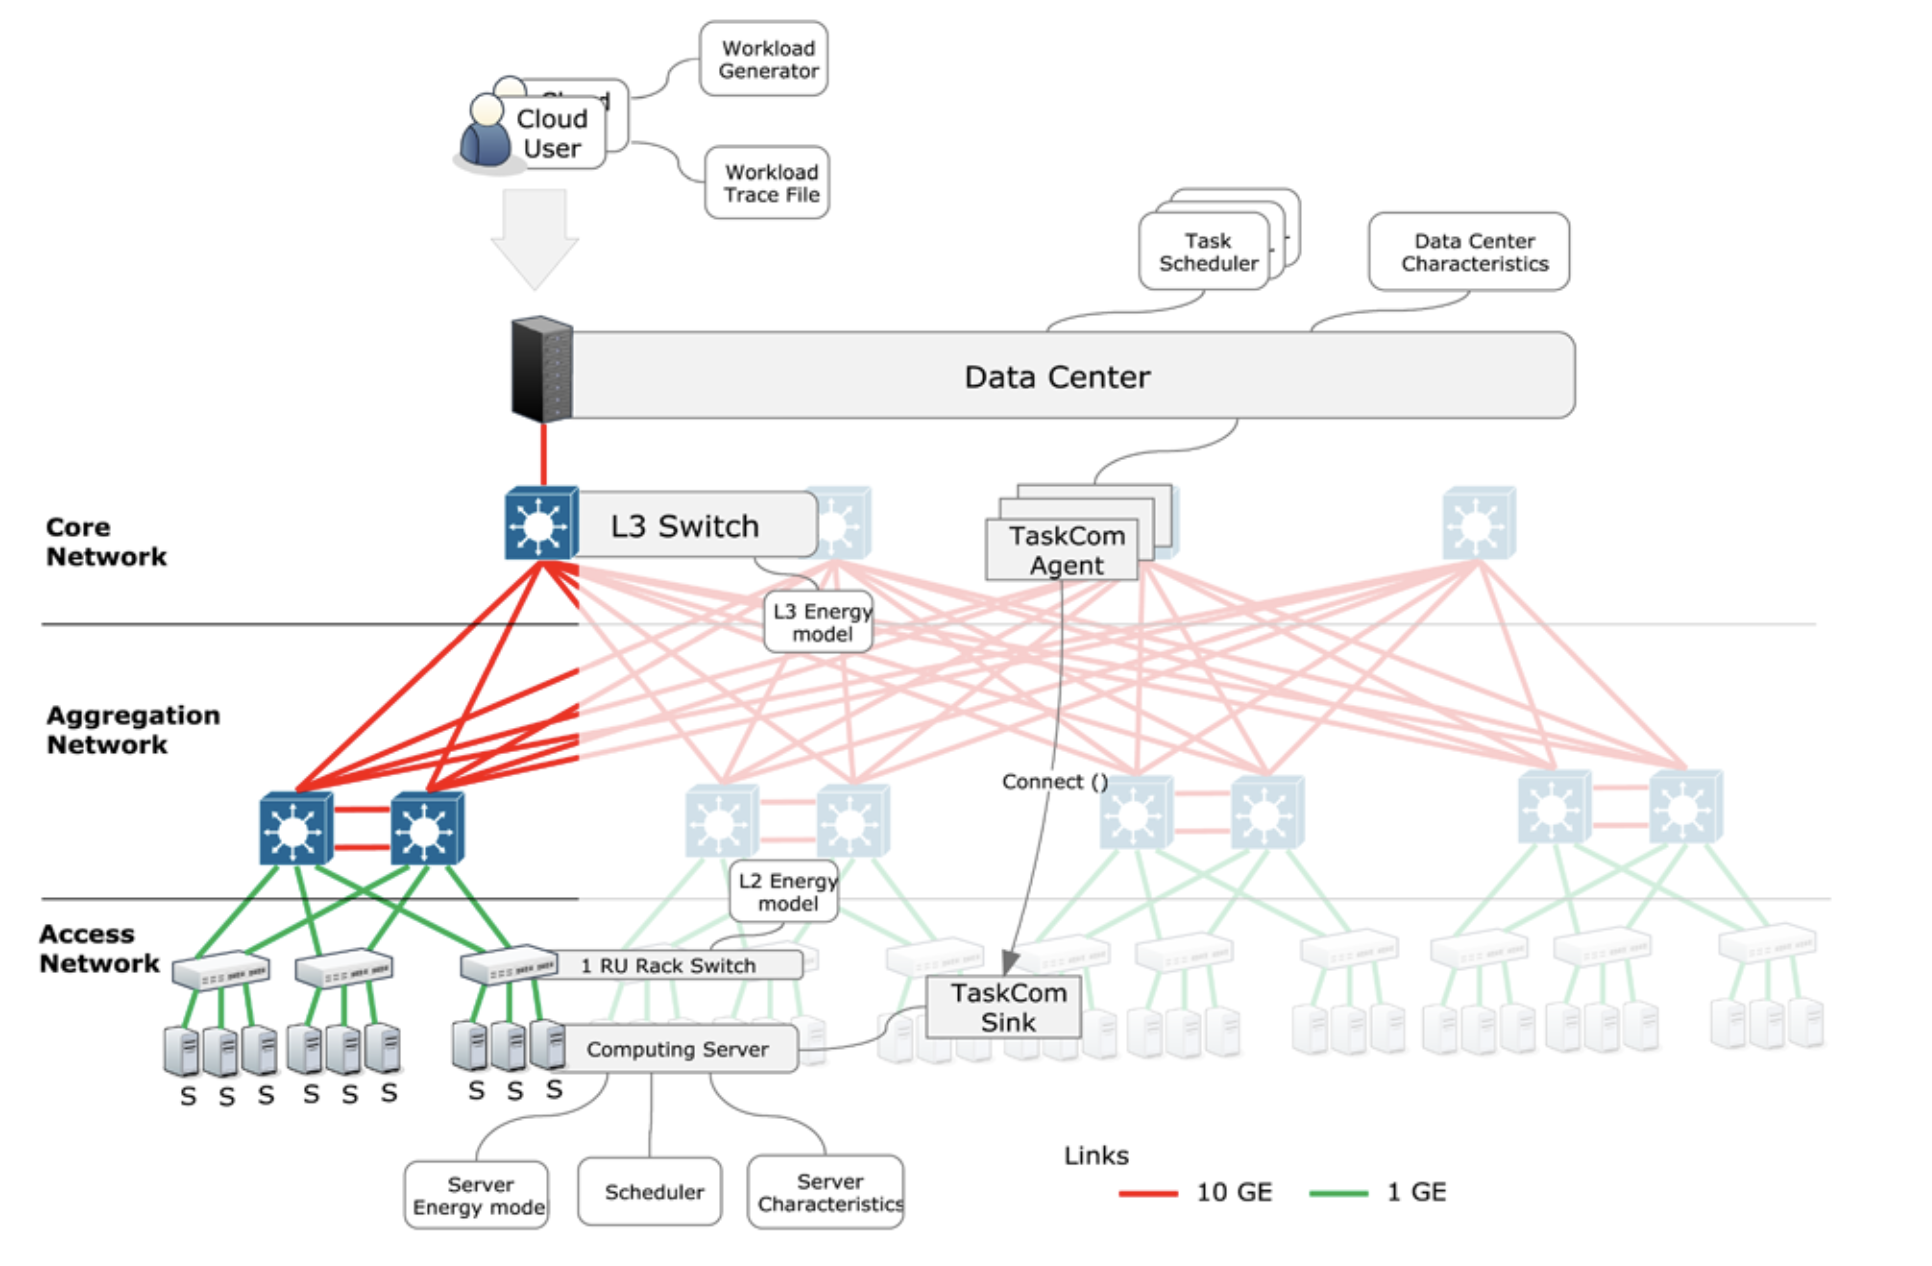
\includegraphics[width=0.5\textwidth]{capitoli/images/greencloud_arch.png}
    \caption{Architecture of the GreenCloud simulation environment}
    \label{fig:greencloud_arch}
\end{figure}
\subsubsection*{iCanCloud}
iCanCloud \cite{nunez2012icancloud} presenta un'apposita \emph{GUI} mediante la quale è possibile configurare il centro di calcolo ed ottenere report grafici. iCanCloud consente di implementare diverse strategie di brokering dando la possibilità di definire diversi broker tra utenti e centro di calcolo. Gli aspetti non contemplati da tale simulatore riguardano il modello energetico e la sicurezza \cite{mansouri2020cloud}. 
\subsubsection*{secCloudSim}
secCloudSim \cite{rehman2014seccloudsim} è un'estensione di iCanCloud che implementa dei semplici meccanismi di sicurezza di cui il suo predecessore è sprovvisto. Tra le diverse funzionalità di sicurezza risulta utile annoverare la presenza di un protocollo di autenticazione e delle \emph{Access Control List} (ACL) mediante le quali è possibile associare specifici privilegi a ciascun utente autenticato. Più in generale secCloudSim fornisce un framework mediante il quale i ricercatori possono sviluppare le caratteristiche di sicurezza come cifratura, decifratura, incapsulamente, autenticazione e privacy. Tuttavia i meccanismi di sicurezza forniti da secCloudSim non sono molto avanzati, per cui i ricercatori non hanno la possibilità di studiare le vulnerabilità dell'infrastruttura \cite{mansouri2020cloud}. 
\subsubsection*{GroudSim}
GroudSim \cite{ostermann2011groudsim} è un simulatore \emph{Java-based} principalmente utilizzato nel contesto di applicazioni scientifiche. Gli sviluppatori hanno la possibilità di importare esperimenti di ASKALON \cite{fahringer2005askalon} all'interno di questo simulatore effettuando simulazioni di applicazioni reali. Questo simulatore pecca in termini di realismo in quanto non permette di configurare una rete realistica in termini di topologia, né risulta essere in grado di scalare. \cite{mansouri2020cloud}.
\subsubsection*{CloudSched}
CloudSched \cite{tian2013toolkit} implementa vari algoritmi di efficienza energetica e diverse strategie di scheduling delle risorse delle macchine fisiche e virtuali al fine di evitare \emph{bottleneck}, dando la possiblità agli sviluppatori di definire algoritmi di scheduling delle risorse \emph{ad-hoc}. CloudSched non tiene conto dei fallimenti nell'esecuzione dei task per cui non risulta possibile prevedere strategie di \emph{fault-tolerance} \cite{mansouri2020cloud}.
\subsubsection*{SimIC}
SimIC \cite{sotiriadis2013simic} ha come \emph{focus} principale l'eterogeneità degli ambienti all'interno dei quali vengono eseguiti gli esperimenti. Gli sviluppatori possono, infatti, definire algoritmi di scheduling \emph{inter-cloud} basandosi su diversi parmetri distribuiti. Le principali limitazioni di tale simulatore risiedono nel fatto che non dia la possibilità di indagare sul consumo energetico né sui controlli relativi al traffico e alle congestioni \cite{mansouri2020cloud}. 
\subsubsection*{SPECI}
SPECI \cite{sriram2009speci} modella gli aspetti relativi alla scalabilità e alle performance dei centri di calcolo dando agli sviluppatori la possiblità di monitorare il comportamento del sistema facendone variare l'architettura. Il simulatore consente, inoltre, di indagare sulle inconsistenze che possono sorgere nel momento in cui si verificano dei guasti. Non vengono, tuttavia, modellati i cambiamenti delle prestazioni delle macchine virtuali durante l'esecuzione nonostante tale fattore abbia una rilevanza particolare negli scenari reali \cite{mansouri2020cloud}.  
\subsubsection*{SCORE}
SCORE \cite{fernandez2018score} si presta alla definizione di algoritmi di scheduling \emph{energy-aware}, ad esempio mediante meccanismi di \emph{shutting-down} e \emph{powering-on}. Risulta, tuttavia, sprovvisto di un modulo di sicurezza che consenta agli sviluppatori di indagarne gli aspetti fondamentali del centro di calcolo \cite{mansouri2020cloud}. 
\subsubsection*{GAME-SCORE}
The GAME-SCORE simulator is an extension of the SCORE simulator written in \emph{Scala}, which uses a combination of discrete-event and multi-agent simulation approaches. Its primary purpose is to simulate energy-efficient IaaS in cloud environments. This simulation tool provides the flexibility to dynamically select energy-efficiency policies from a range of options, allowing for the shutdown of idle machines during runtime. As a practical example, it introduces an algorithm based on the Stackelberg Game that utilizes this capability. However, it's important to note that this simulation tool can accommodate other strategies as well. These strategies can involve the dynamic switching between various energy-efficiency policies and scheduling algorithms. The versatility of this tool enables the implementation of different approaches to optimize energy consumption in simulated environments.
Architecture of GAME-SCORE is shown in figure \ref{fig:gamescore_arch}. It is composed of two modules, described below:
\begin{itemize}
    \item \textbf{Core Simulator Module}: the module responsible for executing the experiments composed of a workload generator, a core engine and a scheduling module;
    \item \textbf{Energy-Efficiency Module}: the module responsible for the implementation of the energy-efficiency policies.
\end{itemize}
It is additionally composed of a special module that implements the Stackelberg Game in order to dynamically switch between energy-efficiency policies. 
\begin{figure}[h]
    \centering
    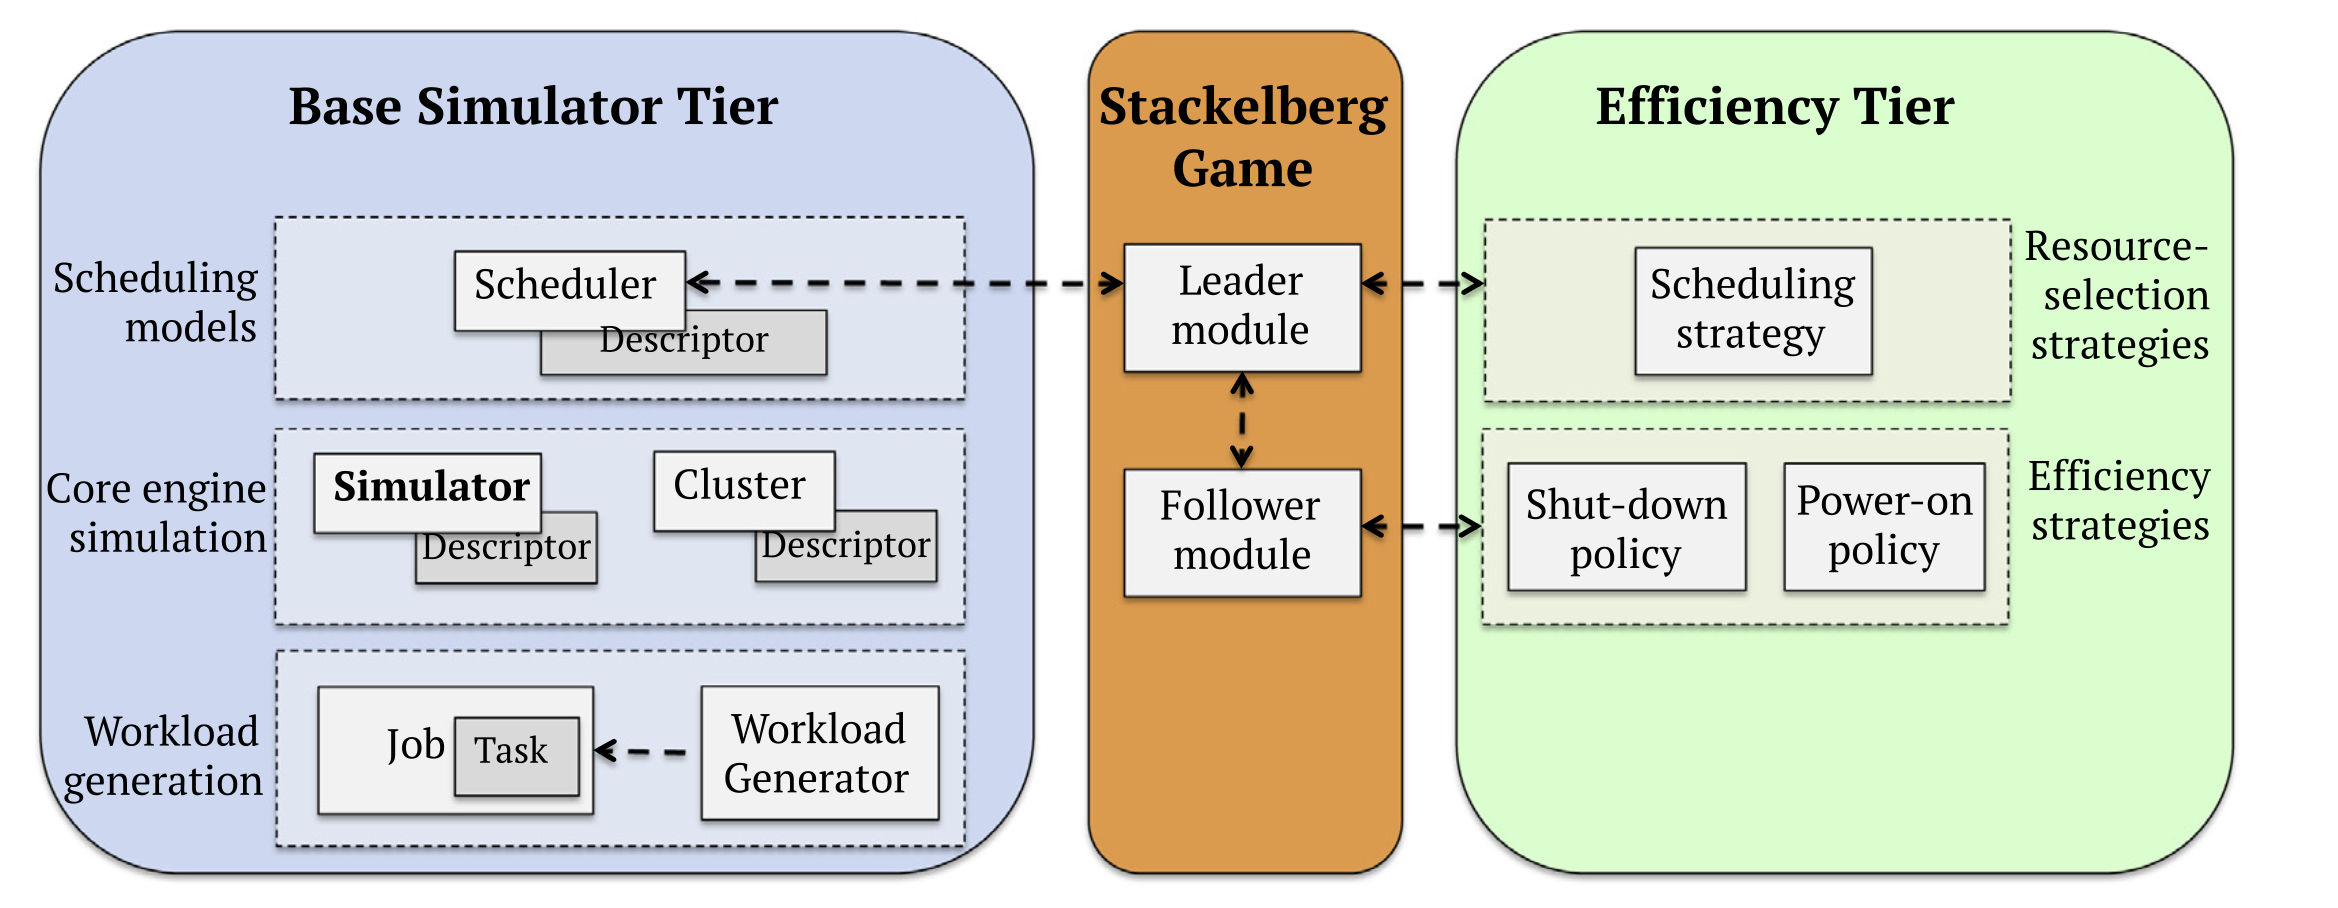
\includegraphics[width=0.5\textwidth]{capitoli/images/gamescore_arch.png}
    \caption{GAME-SCORE architecture}
    \label{fig:gamescore_arch}
\end{figure}
\subsubsection*{DISSECT-CF}
DISSECT-CF \cite{kecskemeti2015dissect} implementa uno schema di condivisione delle risorse del centro di calcolo e un modello energetico dando la possibilità agli sviluppatori di indagare diversi aspetti. Risulta, tuttavia, sprovvisto di un modulo di sicurezza e non dà la possibilità di definire architetture di rete realistiche in quanto mette a disposizione solo un numero limitato di architetture di rete \cite{mansouri2020cloud}.
\subsubsection{ICARO}
ICARO \cite{badii2016icaro} ha come obiettivo principale quello di analizzare i cambiamenti nel carico di un centro di calcolo quando la struttura del carico stesso varia dinamicamente a runtime \cite{khalil2017cloud}. 
\subsubsection{SmartSim}
SmartSim \cite{shiraz2012extendable} simula il comportamento dei dispositivi mobili e delle applicazioni che fanno un uso intensivo delle risorse. \cite{khalil2017cloud}. Grazie a SmartSim è possibile modellare sia i componenti del sistema che il loro comportamento in termini di allocazione e gestione di risorse. \cite{suryateja2016comparative}.
\subsubsection{PICS}
PICS \cite{kim2015pics} è un simulatore progettato per valutare il costo e le prestazioni degli IaaS pubblici tenendo conto di fattori relativi alla gestione delle risorse e allo \emph{scheduling} dei \emph{job}. Tuttavia questo simulatore è sprovvisto di un modello relativo ai costi di comunicazione. \cite{suryateja2016comparative}
\subsubsection{VirtualCloud}

\section{Choice of simulation tool}
Alla luce dei confronti effettuati i diversi tool analizzati si adattano a vari scenari. Ognuno di essi presenta, infatti, punti di forza e punti di debolezza e per le esigenze richieste dallo studio affrontato dal presente lavoro di tesi risulta opportuno privilegiare aspetti relativi al consumo energetico del centro di calcolo, all'accuratezza delle simulazioni e alla sicurezza del centro di calcolo. Dai confronti effettuati si evince che il simulatore che contempla in maniera accurata tali aspetti è GreenCloud, pertanto lo studio proseguirà utilizzando GreenCloud come tool di riferimento per le simulazioni da svolgere. 

\section{}

}

Politiche di spegnimento dei servers
Algoritmi di schedulazione

Controllare la granularità dei consumi 